% -*- mode: latex; mode: linkd; mode: auto-fill; mode: flyspell;-*-
% Index
% (@> "Introduction")
% (@> "Collaboration")
%   (@> "Advantages of collaboration")
%    (@> "Knowledge sharing")
%    (@> "Richer forms of communication")
%    (@> "Share Resources")
%   (@> "Classification of CSCW Systems")

\chapter{Collaborative modelling}
\label{chap-four}

% (@file :file-name "thesis.tex")

% (@* "Introduction")
This chapter introduces the system Coglaborate.
%
The objective of Coglaborate is to provide a collaborative modeling
environment for the cognitive science community. It does so by
mounting ACT-R on the Biobike infrastructure. The system currently
supports collaboration asynchronously. This means that one researcher
can develop a model and share it with his colleague, who can work on
that model separately and share it with other individuals.

% This chapter discusses the advantages provided by a shared environment
% such as Coglaborate. It also tries to provide a framework for the future
% development of Coglaborate, by providing the means that we used to come
% up with the requirements for this system.

This chapter starts off with a discussion of collaborative
systems. This is followed by a discussion of biobike, its objectives,
and which part of the spectrum of collaborative systems it fits
into.

\section{Collaboration}
% (@* "Collaboration")
%explain why is collaboration required. 
Collaboration is the key to building large structures in almost all
human endeavors be it in the fields of either the arts or
sciences. Collaboration permits breaking down large unwieldy tasks
into more manageable chunks of work. It permits sharing of knowledge
and resources. Computer networks have provided us with a means of
communication between users of computers. This as a result has led to
an area of research that studies how computers can help users
communicate their ideas through computers and therefore use computers
as a means of collaboration.  This field is commonly known as Computer
Supported Collaborative Work (CSCW).

\subsection{Advantages of collaboration using computers}
% (@* "Advantages of collaboration")
% Advantages of using computers in collaboration: Describe why you
% need this
Using networks of computers to support collaboration leads to three
outcomes.  Computers assist in sharing knowledge, for example as with
a wiki, freely and easily.  Computers enhance communication by
allowing us to share richer content like video with each
other. Finally networked computers allow us to share resources such as
processing power and storage capacity. Each of these outcomes has its
advantages, discussed in more detail below.

% (@* "Knowledge sharing")
The ability to share knowledge through computers helps us save
time. For example, if a researcher develops a model of some phenomenon
on a computer, that model can be shared with a larger community. Some
other person working on an extension of the project would save the
time taken to build this model in the first place.  And because it is
knowledge being shared, collaboration through computers lends itself
to pedagogy. For instance, consider an author of a textbook. He can
easily create content, such as presentations; he can write programs to
demonstrate concepts; he can share his work on a Web site. This
information can later be used by other student and teachers to learn
more effectively and to improve the way they teach
respectively. Sharing knowledge also implies sharing data. Running
experiments can be time consuming and costly. For example, a
researcher studying weather in one lab could simulate a scenario and
make the data for the same available for others; this saves time and
cost over the entire community of people interested in the phenomena
under study.

% (@* "Richer forms of communication")
Collaboration through the means of computers provides us with richer
forms of communication unavailable to us before, such as audio-based
and video-based communication. As a result we can communicate with
each other more comprehensibly; this in turn avoids transfer of
ambiguous information. For example, we have systems currently that
help us share display screen information.  Such systems can be used by
a customer to clearly communicate his requirements unambiguously to a
vendor, who may be in a different geographical area.

% (@* "Share Resources")
The ability to tie computers together allows us to share
resources. This can be in the form of hardware, where a power server
or servers are shared by many people, or in the form of human
resources, where people from different geographical locations can
collaborate effectively.

% 1) Easier to share knowledge:
%    a) Talk about sharing data,
%    b) code,
%    c) reuse of knowledge
% 2) Communication
%    a) Provides communication: wiki, 
% 3) Repository of knowledge
%    a) Store old knowledge
% 4) Hardware sharing
%    a) More powerful hardware at a common place
%    b) Cost change

\section{Classification of CSCW systems}
% (@* "Classification of CSCW Systems")

According to Rodden~\cite{journals/iwc/Rodden91}, there are two
characteristics of all CSCW systems, namely, the form of interaction
and the geographical nature of the users, as shown in
Figure~\ref{fig:cscw-systems}.

The form of interaction can be described as the method by which users
of a groups working together interact. This could either be
synchronously, where every member of a group contributes in real time,
as in a brain storming process, or asynchronously, where the members
of the group interact with one another over time, not necessarily
contributing simultaneously.  An example of this might be a group of
students collaborating with each other on a homework problem via a
message board.

The geographical nature of the users describes whether the users
interact with each other remotely or locally.  For example, consider
the case of developing the linux kernel: developers and testers worked
with each other on the kernel in geographically disparate locations,
remotely.  Alternatively, users may be co-located, as with the users
of a meeting room system like Colab~\cite{Stefik:1987:BCU}.

\begin{figure}[htp]
  \caption{Classification of CSCW systems\cite{journals/iwc/Rodden91}}
  \label{fig:cscw-systems}
  \centering
  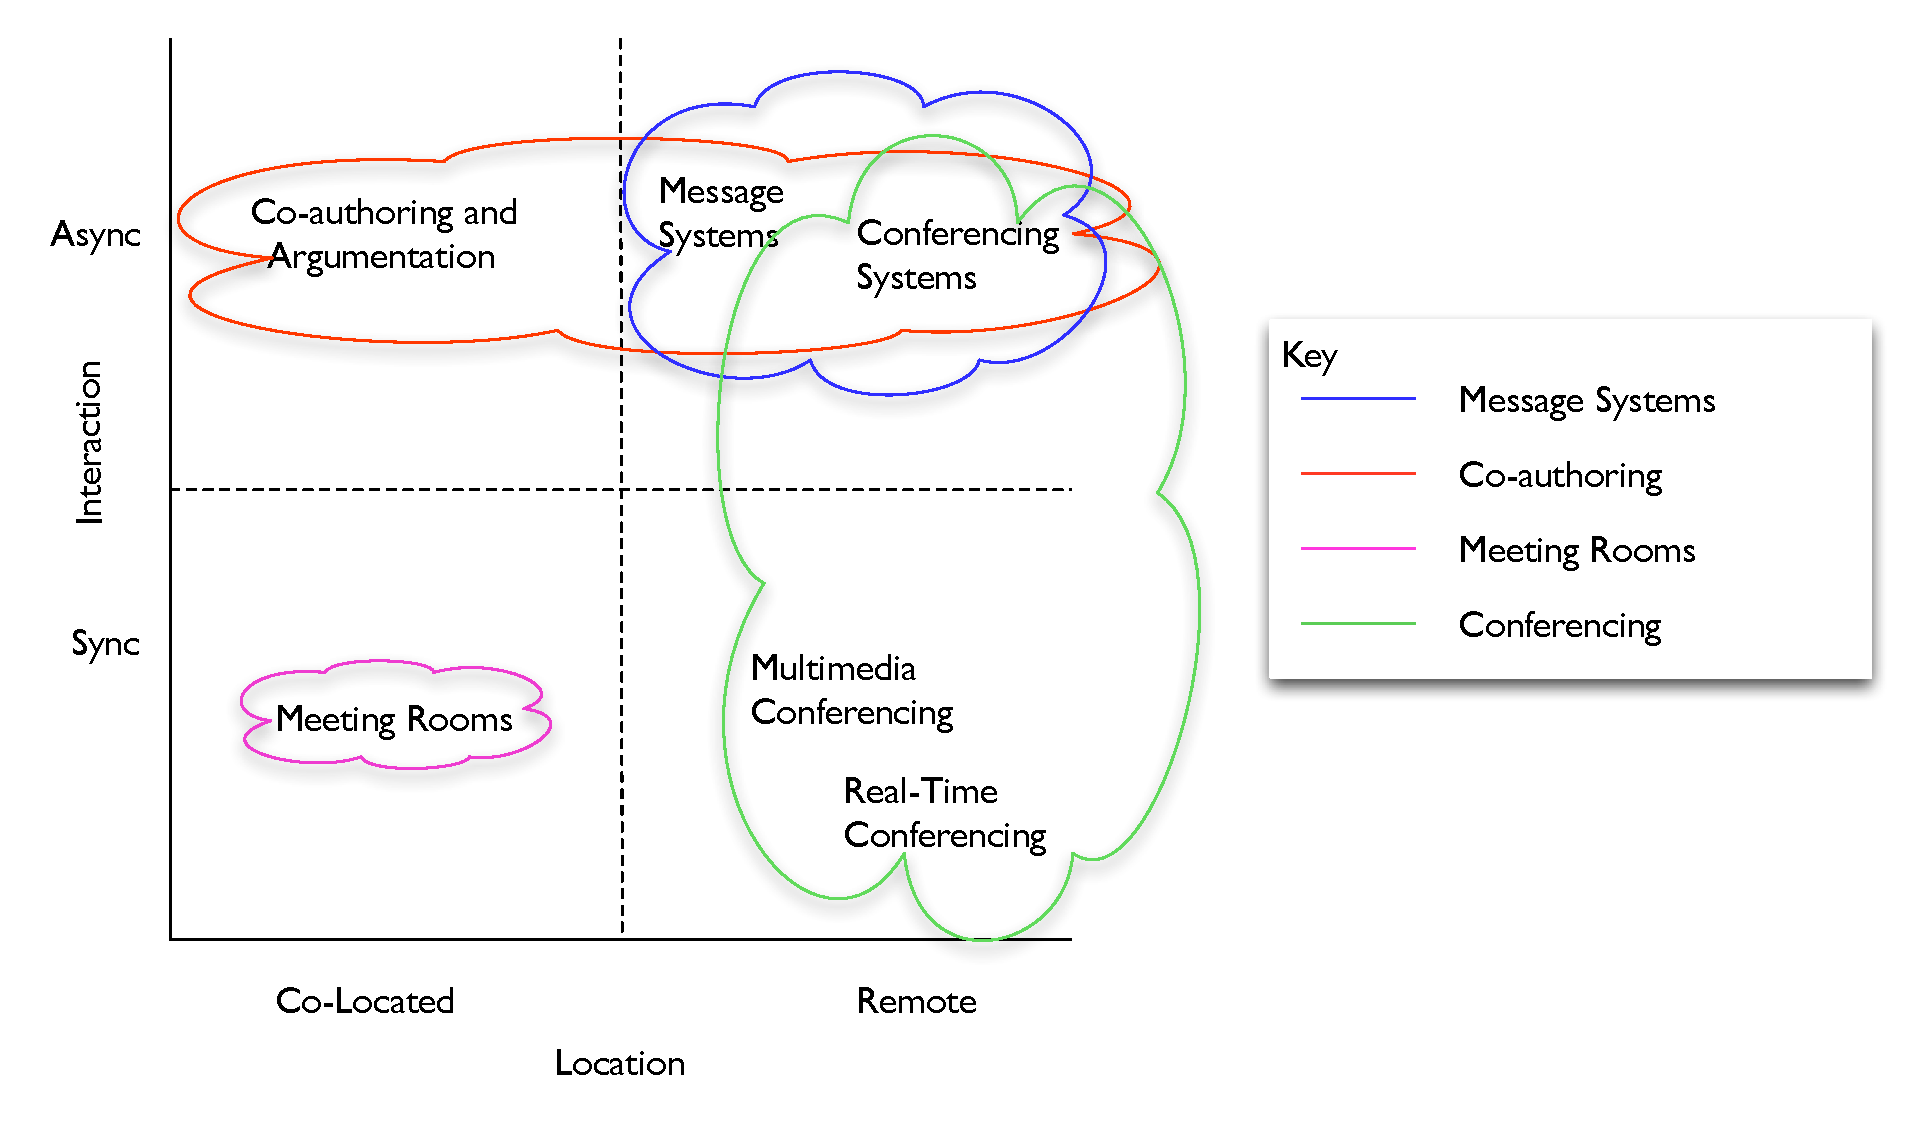
\includegraphics[width=140mm]{CSCWClass.eps}
  \label{CLASS_CSCW}
\end{figure}

\subsection{Message Systems}

Message systems derive their origins from email-based systems. What
differentiates message systems for CSCW from email-based systems is
that such message systems try to attach more semantic data to the
messages they process. Most of these systems use an object model to
represent messages. To instantiate messages the user fills
context-specific data into slots; this data is used by the system to
carry out further processing by the system.  Examples of message
systems for CSCW include COSMOS~\cite{conf/cscw/BowersC88} and
Information Lens~\cite{Malo87a}.

COSMOS represented research being carried out in the European CSCW
community. COSMOS was a project in the UK to design and develop a
configurable message system that supported structured group work. The
system was developed with a focus on specifying the users'
communicative work in the form of participants actions. Group activity
tasks are represented in the system using the concept of
\emph{communication structures}
(CS)~\cite{conf/cscw/BowersC88}. Communication structures are further
described using a structure definition language (SDL). The tasks a
COSMOS system is capable of carrying out are defined by the
communication structures in the system. The COSMOS system also
defines roles for users (or agents), message objects, actions, rules, and
actions in context of the work being carried out. Any communication
activity by the user is instantiated when the user creates an instance
of a communication structure. The user does this by filling in the
data required by the communication structure. Further communication
occurs by an exchange of messages between users, who compose a specific
role specified in the communication structure.

The Information Lens takes a less formal
approach~\cite{journals/iwc/Rodden91}. The aim is to develop
information systems that minimize information overload on the users of
the system caused by the amount of incoming messages. The key ideas
that defined Information lens are


\begin{itemize} 
\item \emph{Use of semi-structured messages to represent data:}
  Messages are represented as a set of semi-structured data called
  frames. A frame is a template that includes information for date,
  time, place, organizer, and any other unstructured data. This idea
  plays an important role because semi-structured messages make it
  easier for the computer to parse messages, according to informal
  studies conducted by the developers of the system~\cite{Malo87a}.
  People do most of their processing on a set of unstructured
  information and thus the use of semi-structured fields, rather than
  more formal structures, enables authors to include more
  context-related information than would otherwise be practical.

\item \emph{Use of production rules:} The system uses sets of
  production rules, each of which might contain multiple levels of
  reasoning that specify how to process messages.

\item \emph{Use of specialized editors for creating and editing
    message templates and productions: } The Information Lens is made
  more usable with multiple editors to create and edit message
  templates and productions.

\item \emph{Use of frame inheritance:} Using frame inheritance in
  messages allows messages to be specialized very easily.

\item \emph{Introduction of the system slowly to the users:} The
  developers believed that the introduction and evolution of a group
  work system is more useful if it is introduced slowly to users.
  Users are encouraged to switch to the system by incremental rewards.
\end{itemize}

The message templates consist of forms having fields where information
could be filled in.  Messages are edited using a display-oriented
editor. The users construct the IF part of a rule by specifying the
conditions that are required to satisfy specific conditions, using
logical operators like {\em and}, {\em or}, and {\em not}. The users
rely on message-handling primitives like {\em move}, {\em delete},
{\em save}, etc. to specify the action to be taken for that message.

\subsection{Conferencing systems}
Conferencing systems were first developed in the 1970s when the US
government was looking for a way to deal with
emergencies. EMISARI~\cite{Hilt78a} (Emergency Management Information
System and Reference Index) was one result of this effort. It consists
of two main ideas that even today form the backbone of current
conferencing systems, as illustrated in Figure~\ref{CONF_SYS}. This
model of communication allows users to interact through a shared
information space, and at the same time it allows users to interact
individually with one another.

\begin{figure}[htp]
  \caption{Communication in a conference system\cite{journals/iwc/Rodden91}}
  \centering
  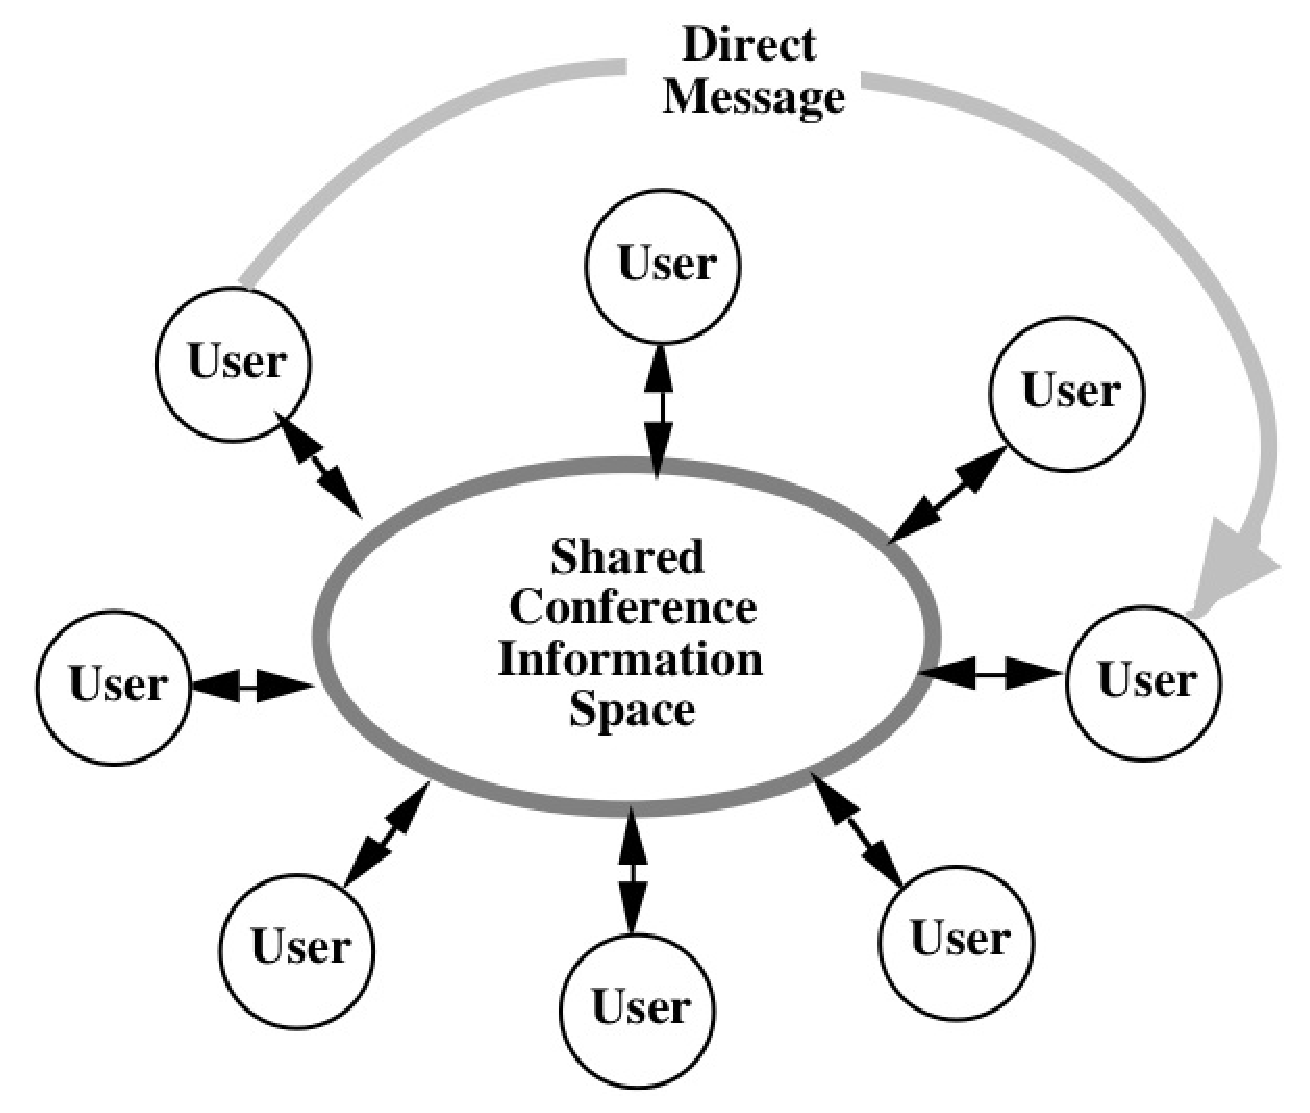
\includegraphics[scale=.5]{ConfSys.eps}
  \label{CONF_SYS}
\end{figure}

% Rodden describes two critical features of the shared information space
% as implemented in conference systems: the type of information
% available to be shared and the form of interaction. The users can use
% the system asynchronously over a long period of time or synchronously
% in real time. With the advent of newer formats of representing data
% the system can use a wide range of media to represent information.

\subsubsection{Traditional conferencing systems}
Traditional conference systems are also extensions of email
systems. The users of a system can subscribe to various conferences
and the system sends messages as comments are posted.  These are
different from mailing lists in that they allow discussions to be
moderated by users.  They also provide flexibility in the way
conferences are created.  Examples of traditional conference systems
include NOTEPAD, by InfoMEDIA Corp, and Confer, a conferencing system
developed at the university of Michigan.

\subsubsection{Real-time conferencing systems}

Real-time conferencing enables an instantaneous transfer of ideas and
flow of information between participants of the conference. Real-time
conferencing is important in situations that require real-time group
participation.  RTCAL~\cite{SG85} was a system developed at the MIT
Laboratory for Computer Science.  It supported scheduling meetings by
building a shared workspace of information from the participants'
calendars.  Although it did not provide a tool that automatically
selects times for meetings, it provides a set of decision support
tools to help schedule meetings.  RTCAL demonstrated a number of
features that are still relevant and applicable to most real time
conferencing systems today, most notable Microsoft Live Meeting.

Real-time conferencing systems may sometime also provide the user with
the facility to share screens. These are called shared screen
systems. Much of the work on shared screen systems are developed on
the work of Colab~\cite{Stefik:1987:BCU}. Yuuguu is a modern example
of an instant screen sharing system.

\subsection{Meeting Rooms Systems}
% Describe meeting room systems. What they support.

% Another factor about meeting room systems

Meeting room systems find their roots in work on Group Decision
Support Systems (GDSS). Kraemer~\cite{KraKin88} cites DeSanctis and
Gallupe\cite{DG85} in a definition of a Group Decision Support System
as ``an interactive computer-based system that facilitates the
solution of unstructured problems by a set of decision makers working
together as a group.'' The eventual aim of such systems is to help
groups improve their decision making process, by providing structure
for the process and a set of tools that help groups to make better
decisions.

More modern meeting room support systems are designed to enable
collaboration between co-located groups of participants.  This is
typically arranged in a meeting room that contains a large projector
along with a number of individual terminals.
Figure~\ref{meeting_room_fig} illustrates this arrangement.

\begin{figure}[htp]
  \caption{Arrangement of a meeting room system\cite{journals/iwc/Rodden91}}
  \centering
  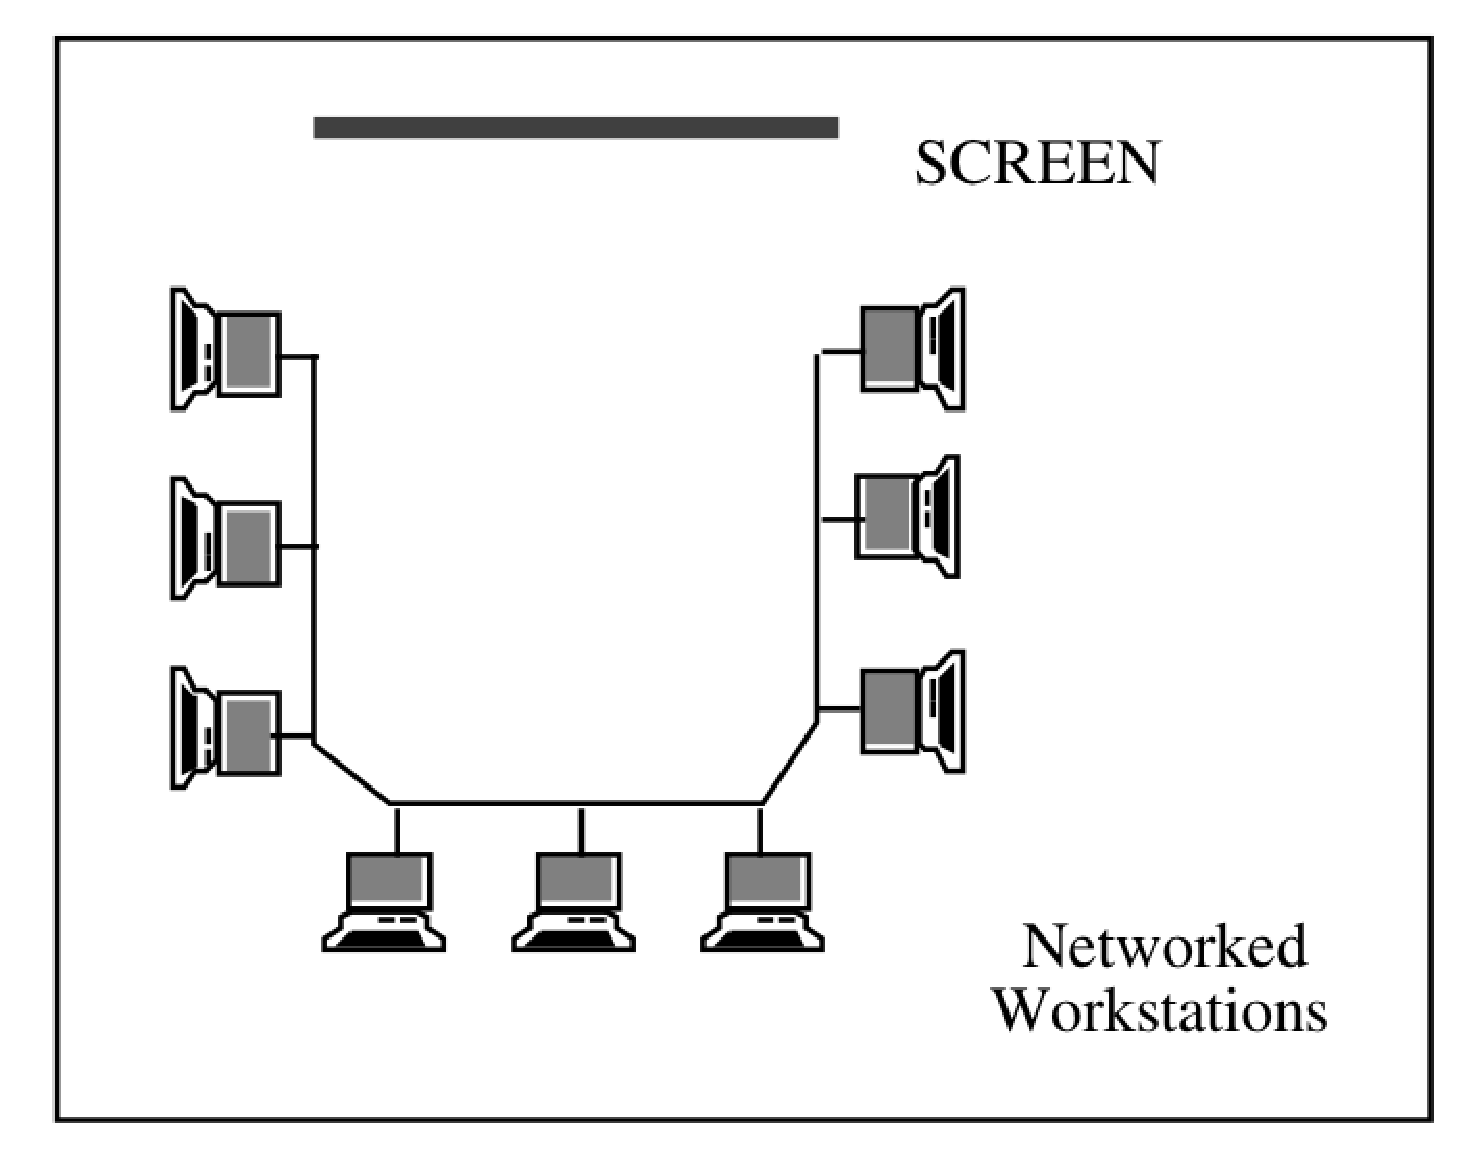
\includegraphics[scale=.5]{meeting_room_sys.eps}
  \label{meeting_room_fig}
\end{figure}

%Describe colab: 

%1) Talk about the objectives

CoLab~\cite{Stefik:1987:BCU} is one of the earliest and most
influential examples of a meeting room system. It aimed to explore the
idea of using computers in meeting rooms to carry out tasks that
generally required media, such as chalk boards. Although the use of
chalkboards and similar media generally helps with group focus, these
media have limitations.  For example, the contents of a standard
chalkboard cannot be reproduced once erased, and rearranging items on
a chalk board is inconvenient.

%2) Features 
CoLab attempted to provide a way around these drawbacks by having a
shared information space where participants of a conference interacted
with one another. This led to investigation of multi-user interfaces,
where users can interact with one another using a computer.  One
concept that resulted from this work was What You See Is What I See
(WYSIWIS): every user sees exactly the same information.  Work on this
concept produced the finding that strict WYSIWIS interfaces are too
limiting.  The designers of CoLab thus opted for a more relaxed
interpretation of WYSIWIS, where every user had private windows in
addition to a display shared with everyone else for interaction.

Since CoLab allowed a number of collaborators to interact with one
another, its basic design led conflicts between individual users
trying to modify the same object at the same time.  As a result the
team experimented with a number of mechanisms to maintain
concurrency~\cite{Stefik:1987:BCU}.

%3) Describe the components -- Not required, these are tools and as
%such do not add to the discussion.
%  3.1) CogNoter
%  3.2) ArgNoter

\subsection{Co-authoring Systems}

A number of projects can be accomplished only by the effort of a
number of authors. Co-authoring systems help support such activity. A
wiki can be considered an example of such a system. Any user can read
an article and, when required, they modify the content of the
article. A wiki also provides space for authors to discuss posted
information via a separate space for comments. A wiki provides version
and configuration control when saving the updates made to a given
document.

\section{Coglaborate}

% Use this section to describe the goals of coglaborate and show which
% class of systems does coglaborate fall under.

Coglaborate, the system developed for this thesis, aims to support
collaboration between cognitive scientists who build computational
models of their work.  Currently these users are restricted to sharing
knowledge through the informal means of annual conferences, workshops,
summer school and model code distributed via web sites.  Coglaborate
is a collaborative modeling environment in which cognitive modeling
researchers can develop and share models.

% Goals of coglaborate
% Provide collaboration for people working in the area of cognitive
% modeling

% Features of coglaborate

Coglaborate currently provides the following features, which are
described in detail in Chapter~\ref{chap-five}:
% Users a provided with a lisp listener where they can evaluate their
% code directly

% The users use a customized version of ACT-R that insulates models
% from colliding with each other when running

% The users can evaluate the model immediately and see the result
% immediately

% Once evaluated any user on the system can search and obtain the code
%   for it from the frame representation of the model.

\begin{itemize}
\item A live lisp listener in a web browser where code can be evaluated.
\item A structured representation for models using frames.
\item A method for sharing and examining models at any level of
  detail.
\end{itemize}

Coglaborate provides support for collaboration by compiling the user's
models into a frame-based representation. These representations are
stored in a common area of the memory of the system. Any user who is
familiar with the name of the model can search for the model and
convert the model to code. This code can then be edited and
recompiled, as a result of this process the original representation is
modified to reflect the change.

Coglaborate can be classified as a co-authoring system. The rationale
behind choosing this classification is that different users can build
the same models incrementally by adding productions or editing
existing models. The following chapter will examine in detail the
design and implementation of the system.
% How does it do it
% Converts all models into frames when evaluated and as a result
% anyone else can search for the frame and manipulate it, re-eval it
% and share it out.

% as a result in its current form Coglaborate is a asynchronous
% co-authoring system because you can have multiple authors working on
% a model.